\documentclass[11pt]{beamer}
\let\Tiny=\tiny
\let\epsilon=\varepsilon
\usepackage{amsmath}
\usepackage{amsfonts}
\usepackage{amssymb}
\usepackage{graphicx}
\usepackage{array}
\usepackage{tikz}
\usepackage{framed}

\definecolor{cherryred}{RGB}{214,31,74}
\definecolor{sandiasilver}{RGB}{204,204,204}
\definecolor{lightblue}{RGB}{240,245,255}

\usecolortheme[named=cherryred]{structure}
\usefonttheme[onlymath]{serif}
\setbeamertemplate{navigation symbols}{}
\setbeamertemplate{blocks}[shadow=true]
\setbeamersize{sidebar width left=0.2cm}
\setbeamercolor{sidebar}{bg=sandiasilver}
\setbeamercolor{frametitle}{fg=white, bg=cherryred}
\setbeamertemplate{theorems}[numbered]


\author{David E. Weirich}
\title{Neural Networks: \\ The Hard Way}
\date{\today}

\newcommand{\R}{\mathbb{R}}
\newcommand{\C}{\mathbb{C}}
\newcommand{\Z}{\mathbb{Z}}
\newcommand{\D}{\mathcal{D}}
\newcommand{\A}{\mathcal{A}}
\newcommand{\B}{\mathfrak{B}}
\newcommand{\Dh}{\tilde{\mathcal{D}}}

\newcommand{\supp}{\operatorname{Support}}
\newcommand{\ch}{\operatorname{ch}}
\newcommand{\proj}{\operatorname{Proj}}
\newcommand{\spn}{\operatorname{span}}
\newcommand{\quadr}{\operatorname{Quad}}
\newcommand{\qak}{Q_\alpha^k}
\newcommand{\one}{\textbf{1}} % Get the better looking one working!

\newcommand{\mean}[2]{\langle #2 \rangle_{#1}}

\newtheorem{conjecture}[theorem]{Conjecture}

\newcommand{\zak}{z_\alpha^k}

\newcommand{\bfred}[1]{{\color{cherryred} \textbf{#1}}}
\begin{document}

\begin{frame}
\titlepage
\end{frame}

\begin{frame}{Talk Objectives}

\begin{itemize}
\item Understand the mathematical basis for artifical neural networks.

\item Use that knowledge to design and build a neural network without relying on preexisting ML frameworks.
\end{itemize}

Or more consicely...

\textbf{Learn Neural Networks THE HARD WAY}

\end{frame}

\begin{frame}{Disclaimer}
\begin{center}
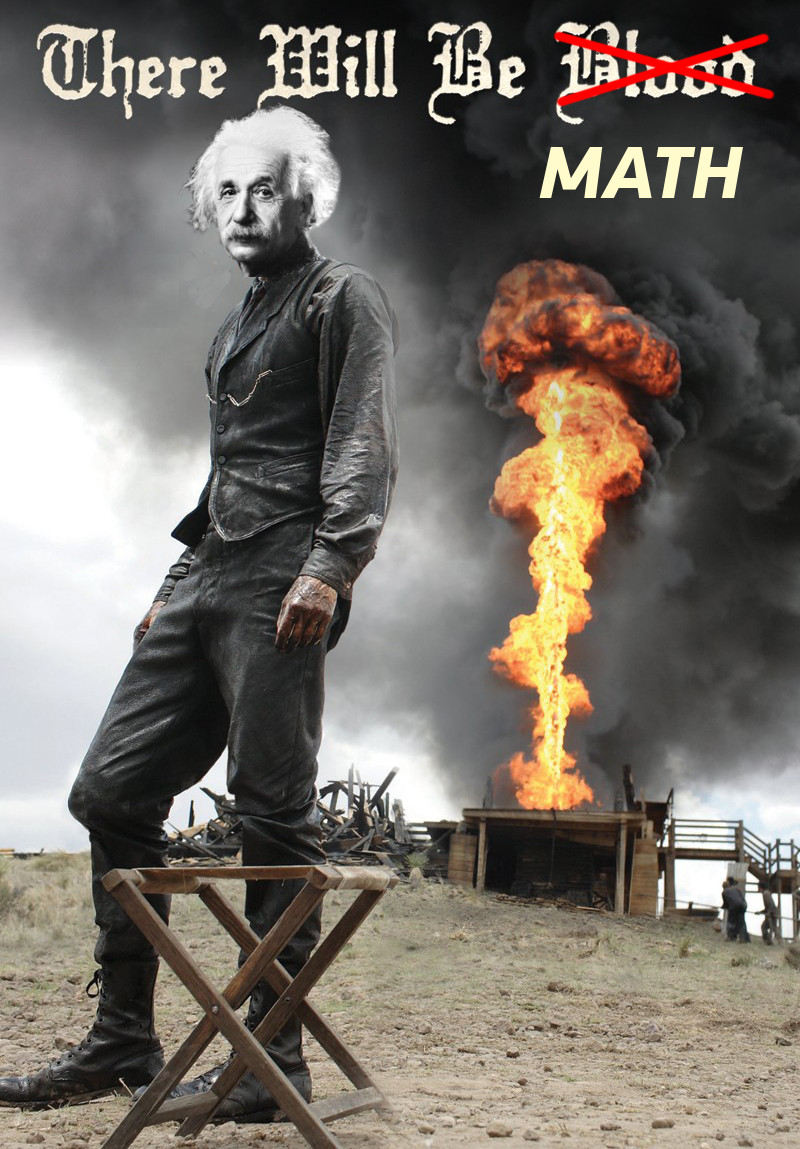
\includegraphics[scale=0.18]{ThereWillBeMath}
\end{center}
\end{frame}

\section{What are these Neural Networks Things?}

\begin{frame}{What are Neural Networks?}
Q: What is a neural network?

\bigskip 

A: \emph{A neural network is this super confusing thing that is kind of like an artifical brain.}

\bigskip 

Q: Why do we care?

\bigskip 

A: \emph{It can learn anything, do anything, and no one understands them.}
\end{frame}

\begin{frame}{Why the "hard way"??? I prefer easy!}

What do I mean by "the hard way"?

Doing things the hard way means teaching you how to teach yourself.

\end{frame}

\begin{frame}{The Problem}

We wish to approximate a function given a finite collection of known inputs and outputs.

\bigskip

$$||F - \widehat{F}|| < \epsilon$$

\bigskip

Here $F$ is the true function, and $\widehat{F}$ is our approximation.
\end{frame}

\begin{frame}{Neurons}

\begin{center}
\begin{figure}
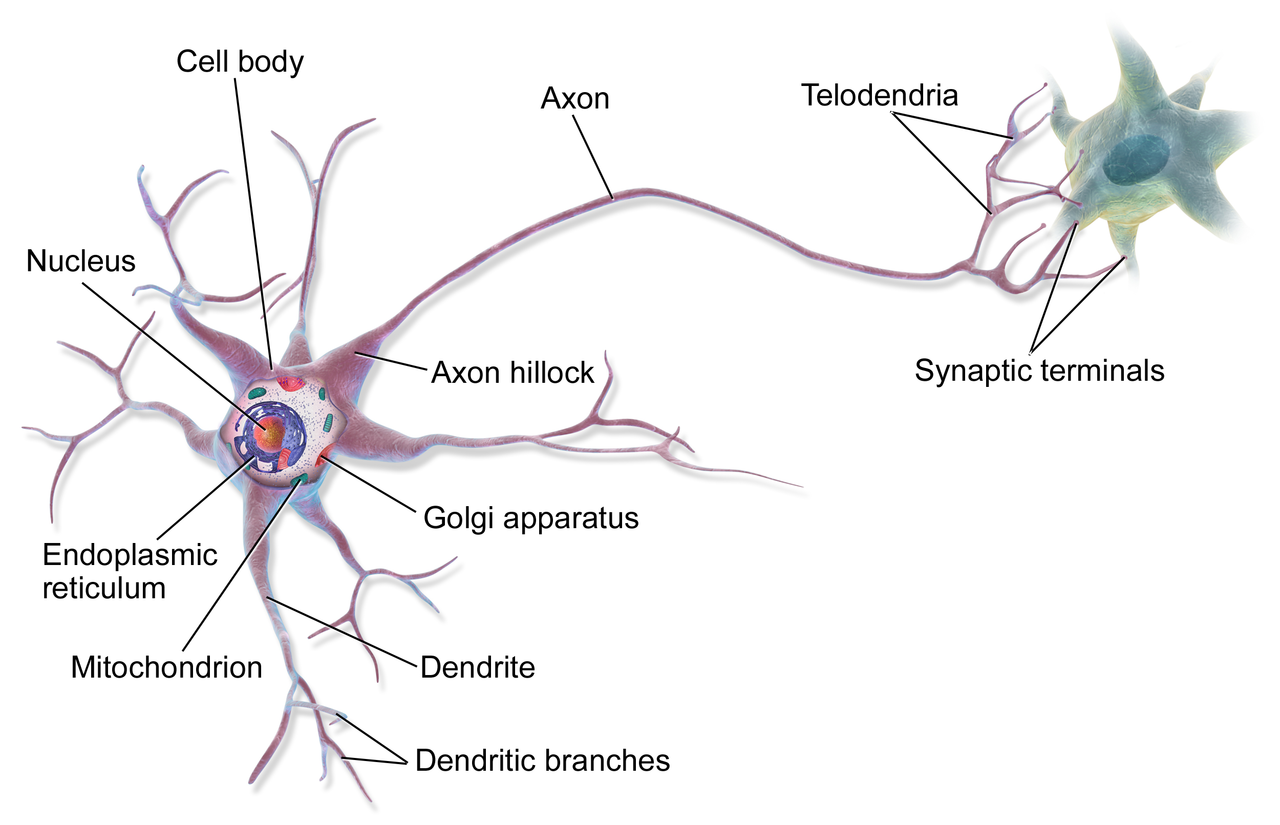
\includegraphics[scale=0.1]{Blausen_0657_MultipolarNeuron}
\caption{A neuron. These things are involved somehow? (Source: Wikipedia)}
\end{figure}
\end{center}
	
\end{frame}

\begin{frame}{Pictures that look like this}

\begin{center}
\begin{figure}
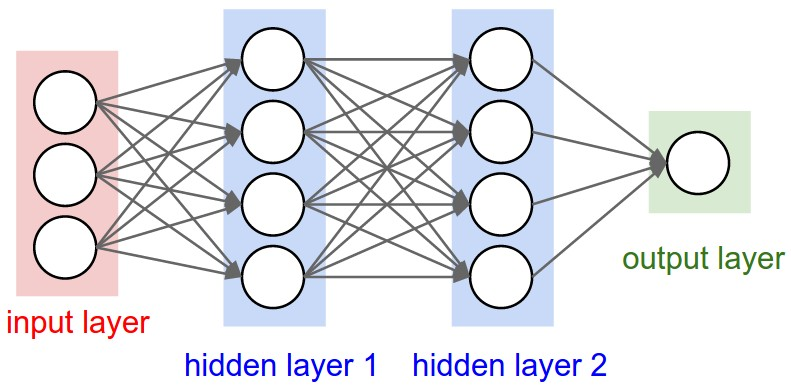
\includegraphics[scale=0.2]{0_IlHu39jf2c7QC4kn}
\hspace{5mm}
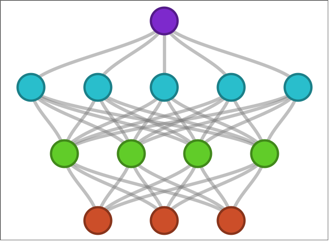
\includegraphics[scale=0.2]{topdown}

\vspace{5mm}

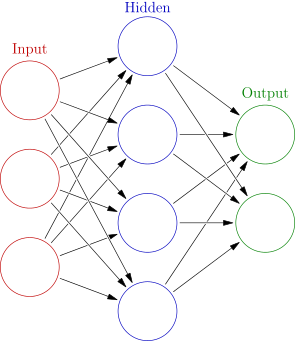
\includegraphics[scale=0.25]{296px-Colored_neural_network}
\hspace{5mm}
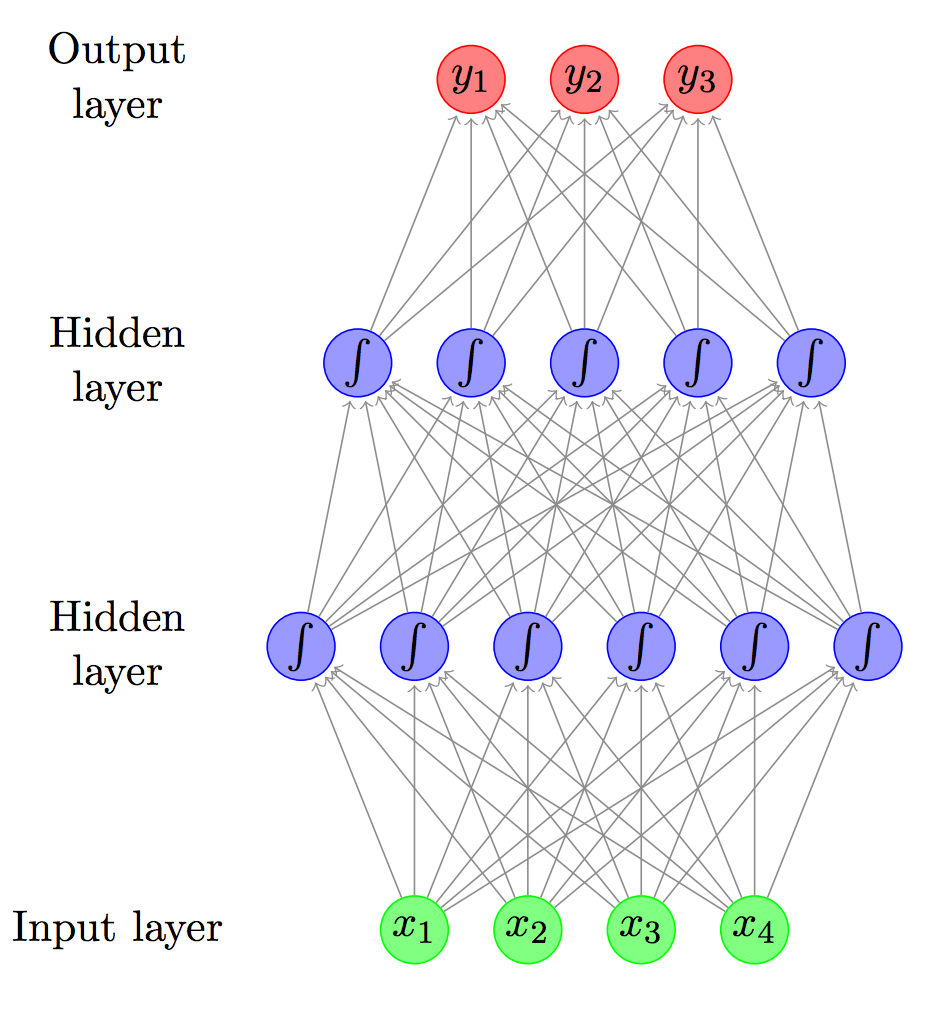
\includegraphics[scale=0.15]{Feed-forward-neural-network-with-two-hidden-layers}
\caption{Some diagrams with circles and arrows.}
\end{figure}
\end{center}

\end{frame}

\begin{frame}{Digits}
\begin{center}

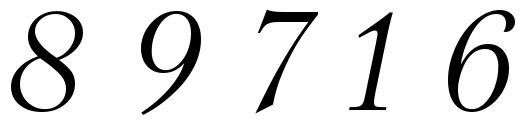
\includegraphics[scale=0.5]{digits}

\pause

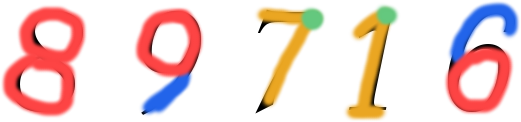
\includegraphics[scale=0.5]{digits2}

\pause

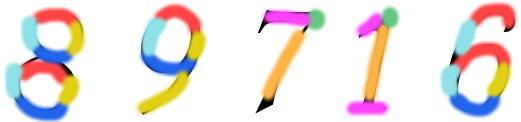
\includegraphics[scale=0.5]{digits3}
\end{center}
\end{frame}

\begin{frame}{The $\Sigma$exy Way}
Let's take a look at the math under the hood:
\begin{align*}
x &= \left[\begin{array}{c}
x_1 \\
x_2 \\
\vdots \\
x_N
\end{array}\right] \\
\widehat{y} &= \widehat{F}(x) = W_2\sigma(W_1\sigma(W_0x + b_0) + b_1) + b_2
\end{align*}

where $W_i$ is a weight matrix, $b_i $ is a bias vector, and $\sigma$ is an activation function.
\end{frame}

\begin{frame}{Breaking that down}

\begin{align*}
z_0 &:= W_0x + b_0 \\
a_0 &:= \sigma(z_0) \\
z_1 &:= W_1a_0 + b_1 \\
a_1 &:= \sigma(z_1) \\
&\vdots \\
\widehat{y} &:= W_n a_{n-1} + b_n
\end{align*}

\end{frame}

\begin{frame}{Universal Approximation Theorem}
\begin{theorem}[Cybenko (1989), Hornik (1991)]
Let $\sigma$ be a nonconstant, bounded, and monotoncally increasing function.
Given any $\epsilon > 0$ and any continuous function $F$ defined on a compact subdomain $\Omega$ of $\R^n$ there exists a constant $N$, real constants $v_i$ and $b_i$, and real vectors $w_i$ such that we may define
$$\widehat{F}(x) := \sum_{i = 1}^N v_i \sigma(w_i^T \cdot x + b_i)$$
with
$$\left|F(x) - \widehat{F}(x)\right| < \epsilon$$
for all $x$ in $\Omega$.
\end{theorem}
\end{frame}

\section{Training}
\begin{frame}{Okay, fine, I get it. But how do I set those weights?}

For $M$ observations $(x_i, y_i)$, define a loss function

\begin{align*}
J(y_i, \widehat{y}) &:= \frac{1}{2M}\sum_{i =1}^N (y - \widehat{y})^2 \\
&= \frac{1}{2M}\sum_{i =1}^N \left(y - \widehat{F}(x_i)\right)^2 \\
&= \frac{1}{2M}\sum_{i =1}^N \left(y - \widehat{F}(x_i; W, b)\right)^2 
\end{align*}
Now we just have to minimize the loss!
\end{frame}

\begin{frame}{The Gradient}
Recall from multivariable calculus that the \emph{gradient} is a vector which points in the direction of steapest assent on a surface.
\begin{center}
\begin{figure}
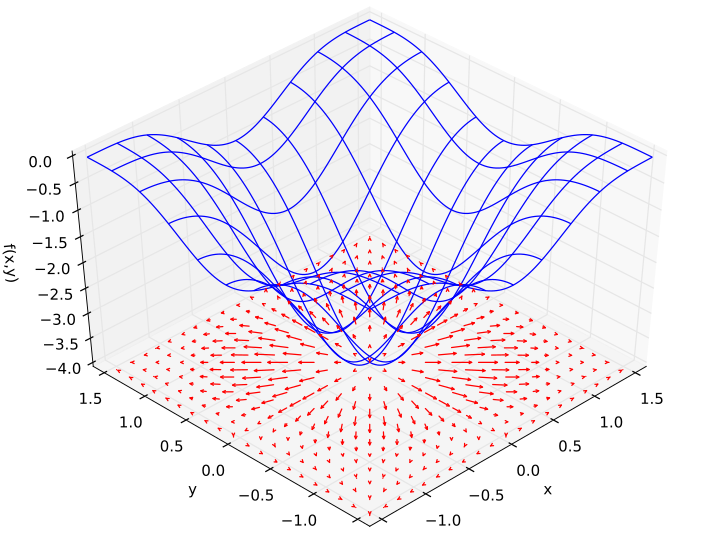
\includegraphics[scale=0.25]{720px-Gradient_Visual}
\caption{A function of two variables, with it's gradient.}
\end{figure}
\end{center}
\end{frame}

\begin{frame}{The Game Plan}
\begin{itemize}
\item We start by setting the weights and biases of the NN randomly.
\item Calculate the gradient of the loss function $J$ with respect to these parameters.
\item Take a small step in the direction of the negative gradient.
\item Repeat untill the error is acceptable.
\end{itemize}
\end{frame}

\section{The Code}

\begin{frame}{WE'LL DO IT LIVE}
\begin{center}

\includegraphics[scale=0.3]{114486a48d800d14f972cb0e74f7b0d9}

WE'LL DO IT LIVE!
\end{center}
\end{frame}

\section{End}

\begin{frame}
\begin{center}
Thank you! :)
\end{center}
\end{frame}

\end{document}
